\documentclass{standalone}
\usepackage{tikz}
\begin{document}
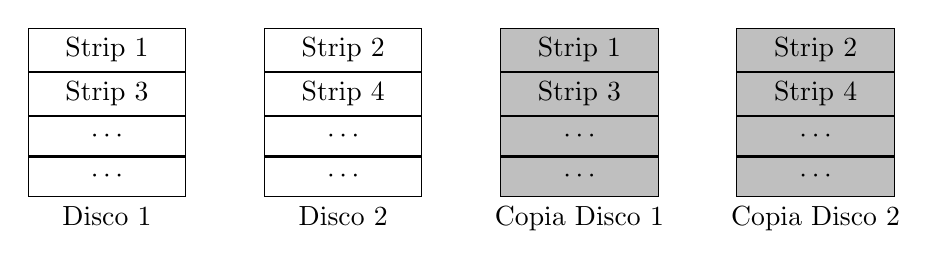
\begin{tikzpicture}
    \draw

    (0,0)node[rectangle, draw, minimum width=2cm, minimum height=0.5cm,anchor=north](a){Strip 1}
    (a.south)node[rectangle, draw, minimum width=2cm, minimum height=0.5cm,anchor=north](a){Strip 3}
    (a.south)node[rectangle, draw, minimum width=2cm, minimum height=0.5cm,anchor=north](a){$\cdots$}
    (a.south)node[rectangle, draw, minimum width=2cm, minimum height=0.5cm,anchor=north](a){$\cdots$}
    (a.south)node[below]{Disco 1}
    
    (3,0)node[rectangle, draw, minimum width=2cm, minimum height=0.5cm,anchor=north](a){Strip 2}
    (a.south)node[rectangle, draw, minimum width=2cm, minimum height=0.5cm,anchor=north](a){Strip 4}
    (a.south)node[rectangle, draw, minimum width=2cm, minimum height=0.5cm,anchor=north](a){$\cdots$}
    (a.south)node[rectangle, draw, minimum width=2cm, minimum height=0.5cm,anchor=north](a){$\cdots$}
    (a.south)node[below]{Disco 2}


    (6,0)node[rectangle,fill=lightgray, draw, minimum width=2cm, minimum height=0.5cm,anchor=north](a){Strip 1}
    (a.south)node[rectangle,fill=lightgray, draw, minimum width=2cm, minimum height=0.5cm,anchor=north](a){Strip 3}
    (a.south)node[rectangle,fill=lightgray, draw, minimum width=2cm, minimum height=0.5cm,anchor=north](a){$\cdots$}
    (a.south)node[rectangle,fill=lightgray, draw, minimum width=2cm, minimum height=0.5cm,anchor=north](a){$\cdots$}
    (a.south)node[below]{Copia Disco 1}
    
    (9,0)node[rectangle,fill=lightgray, draw, minimum width=2cm, minimum height=0.5cm,anchor=north](a){Strip 2}
    (a.south)node[rectangle,fill=lightgray, draw, minimum width=2cm, minimum height=0.5cm,anchor=north](a){Strip 4}
    (a.south)node[rectangle,fill=lightgray, draw, minimum width=2cm, minimum height=0.5cm,anchor=north](a){$\cdots$}
    (a.south)node[rectangle,fill=lightgray, draw, minimum width=2cm, minimum height=0.5cm,anchor=north](a){$\cdots$}
    (a.south)node[below]{Copia Disco 2}
    ;
\end{tikzpicture}
\end{document}